% !Mode:: "TeX:UTF-8"

\def\xuewei{Doctor} % 默认
\documentclass[cs4size,openany,oneside,UTF8,nofonts]{ctexbook}
% \usepackage[a4paper,text={160true mm,234true mm},top=30.5true mm,left=25true mm,head=5true mm,headsep=2.5true mm,foot=8.5true mm]{geometry}
\usepackage[a4paper,text={170true mm,246.2true mm},top=25.4true mm,left=20true mm,head=5true mm,headsep=2.5true mm,foot=7.5true mm]{geometry}
\usepackage{ccaption}
\usepackage{booktabs}
\usepackage{longtable}
\usepackage{caption}
\usepackage{amsmath}
\usepackage{amssymb}
\usepackage{mathtools}
\usepackage{bigints}
\usepackage{bm}
\usepackage{txfonts}
\usepackage{graphicx}
\usepackage{enumitem}
\usepackage{fancyhdr}
\usepackage{ntheorem}
\usepackage{titlesec}
\usepackage{titletoc}                   % 控制目录的宏包
\usepackage{subfigure}
\usepackage{tabularx}
\usepackage[sort&compress,numbers]{natbib}
% \usepackage[boxed,linesnumbered,algochapter]{algorithm2e}	
\usepackage[ruled,linesnumbered]{algorithm2e}
% \usepackage{algorithmic}
\usepackage{listings}
\usepackage{lmodern}
\usepackage{tcolorbox}
\usepackage{tikz}
%
\usetikzlibrary{calc}
\lstset{ columns=flexible, breaklines=true }

\usepackage[xetex,
            bookmarksnumbered=true,
            bookmarksopen=true,
            colorlinks=false,
            pdfborder={0 0 1},
            citecolor=blue,
            linkcolor=red,
            anchorcolor=green,
            urlcolor=blue,
            breaklinks=true,
            naturalnames  %与algorithm2e宏包协调
            ]{hyperref}
\defaultfontfeatures{Mapping=tex-text}
\xeCJKsetemboldenfactor{1}%只对随后定义的CJK字体有效
\setCJKfamilyfont{hei}{SimHei}
\xeCJKsetemboldenfactor{4}
\setCJKfamilyfont{song}{SimSun}
\xeCJKsetemboldenfactor{1}
\setCJKfamilyfont{fs}{FangSong}
\setCJKfamilyfont{kai}{KaiTi}
\setCJKfamilyfont{li}{LiSu}
\setCJKfamilyfont{xw}{STXinwei}
\setCJKmainfont{SimSun}
\setCJKsansfont{SimHei}
\setmainfont{Times New Roman}
\setsansfont{Arial}
\newcommand{\heiti}{\CJKfamily{hei}}% 黑体   (Windows自带simhei.ttf)
\newcommand{\songti}{\CJKfamily{song}}    % 宋体   (Windows自带simsun.ttf)
\newcommand{\fs}{\CJKfamily{fs}}        % 仿宋体 (Windows自带simfs.ttf)
\newcommand{\kaishu}{\CJKfamily{kai}}      % 楷体   (Windows自带simkai.ttf)
\newcommand{\li}{\CJKfamily{li}}        % 隶书   (Windows自带simli.ttf)
\newcommand{\xw}{\CJKfamily{xw}}        % 隶书   (Windows自带simli.ttf)
\newfontfamily\arial{Arial}
\newfontfamily\timesnewroman{Times New Roman}
\setCJKfamilyfont{hwxk}{STXingkai}             %使用STXingkai华文行楷字体
\newcommand{\xingkai}{\CJKfamily{hwxk}}


\newcommand{\yihao}{\fontsize{26pt}{26pt}\selectfont}       % 一号, 1.倍行距
\newcommand{\xiaoyi}{\fontsize{24pt}{24pt}\selectfont}      % 小一, 1.倍行距
\newcommand{\erhao}{\fontsize{22pt}{1.25\baselineskip}\selectfont}       % 二号, 1.倍行距
\newcommand{\xiaoer}{\fontsize{18pt}{18pt}\selectfont}      % 小二, 单倍行距
\newcommand{\sanhao}{\fontsize{16pt}{16pt}\selectfont}      % 三号, 1.倍行距
\newcommand{\xiaosan}{\fontsize{15pt}{15pt}\selectfont}     % 小三, 1.倍行距
\newcommand{\sihao}{\fontsize{14pt}{14pt}\selectfont}       % 四号, 1.0倍行距
\newcommand{\xiaosi}{\fontsize{12pt}{12pt}\selectfont}      % 小四, 1.倍行距
\newcommand{\wuhao}{\fontsize{10.5pt}{10.5pt}\selectfont}   % 五号, 单倍行距
\newcommand{\xiaowu}{\fontsize{9pt}{9pt}\selectfont}        % 小五, 单倍行距

\newcommand\litem[1]{\item{\heiti#1\hspace{1.5em}}}

\newenvironment{listitem}{\begin{enumerate}[label={(\arabic*)},itemindent=2em]}{\end{enumerate}}

% \usepackage[boxed,linesnumbered,algochapter]{algorithm2e}  % 算法的宏包,注意宏包兼容性,先后顺序为float、hyperref、algorithm(2e),否则无法生成算法列表
\renewcommand{\algorithmcfname}{算法}

%\usepackage{tikz,mathpazo}

%\usetikzlibrary{shapes.geometric, arrows}

\newcommand{\citeayu}[1]{\citeauthor{#1}~(\citeyear{#1})\citeup{#1}}

\begin{document}

\titleformat{\chapter}{\center\xiaoer\hei}{\chaptertitlename}{0em}{}
\titlespacing{\chapter}{0pt}{0.5\bseieskip}{0.5\bseieskip}
\titleformat{\section}{\xiaosan\hei}{\thesection}{0em}{}
\titlespacing{\section}{0pt}{0.5\bseieskip}{0.5\bseieskip}
\titleformat{\subsection}{\sihao\hei}{\thesubsection}{0em}{}
\titlespacing{\subsection}{0pt}{0.5\bseieskip}{0.5\bseieskip}
\titleformat{\subsubsection}{\xiaosi\hei}{\thesubsubsection}{0em}{}
\titlespacing{\subsubsection}{0pt}{0pt}{0pt}

\newif\ifxueweidoctor
\newif\ifxueweimaster
\def\temp{Doctor}
\ifx\temp\xuewei
  \xueweidoctortrue  \xueweimasterfalse
\fi
\def\temp{Master}
\ifx\temp\xuewei
  \xueweidoctorfalse  \xueweimastertrue
\fi

\input{format}
% !Mode:: "TeX:UTF-8"

\affil{计算机科学与技术}
\subject{计算机应用技术}
\researchdirection{xxxxx}
\author{陈xx}
\supervisor{陈xx \enspace 教授}
% \assosupervisor{副导名}%若无副导师,请屏蔽掉此句
% \cosupervisor{联导名}%若无联合导师,请屏蔽掉此句
\date{2019年12月25日}
\stuno{BA1xxxxxxxx}
\bdate{2004年5月}

\ifxueweidoctor
  \title{基于xxxxxxxxxxx} %论文题目
  \titlesec{xxxxx研究与实现}

\makecover
\clearpage
\setcounter{page}{1} 
\zihao{-4}
% \tableofcontents    % 中文目录
% \chapter*{基于xxxxxxxxxxxxxxxxxx研究与实现}

%\animategraphics[height=2.8in,autoplay,loop,controls]{12}{animate_}{0}{22}
% \input{body/figures}
% \input{body/tables}
% \input{body/equations}
% \input{body/others}
\section{选题依据}

%%%%%%%%%%%% 画框, 每页自己调节
\begin{tikzpicture}[overlay,remember picture]
  \draw [line width=0.8pt]
      ($ (current page.north west) + (1.8cm,-3.5cm) $)
      rectangle
      ($ (current page.south east) + (-1.8cm,2.5cm) $);
\end{tikzpicture}
%%%%%%%%%%%% 画框, 每页自己调节

图片例子
\begin{figure}[htbp]
  \centering
  \includegraphics[width = 0.7\textwidth]{rgbd_1.png}
  \caption{图片例子}\label{图片例子}
  \vspace{-1em}
\end{figure}

算法例子
\begin{algorithm}
  \caption{算法例子}
  \label{alg111}
  Initialize policy network $\pi_\theta$ and value function $V_\phi (s_t)$.

  \For{epoch $ = 1,2...,$}
  {
          \textit{// ...}

          $\pi_{old} \leftarrow \pi_{\theta}$

          \textit{// Update policy network}
          
          \For{$m = 1,...,E_{\pi}$}
          {
                  $L^{PPO}(\theta) = \sum_{t=1}^{T_{max}}{min(\frac{\pi_{\theta}(a_{i}^{t}|o_{i}^{t})}
                  {\pi_{old}(a_{i}^{t}|o_{i}^{t})}\hat{A}_{i}^{t}, 
                  clip(\frac{\pi_{\theta}(a_{i}^{t}|o_{i}^{t})}{\pi_{old}(a_{i}^{t}|o_{i}^{t})},1-\varepsilon ,1+\varepsilon )
                  \hat{A}_{i}^{t})}$

                  \If {KL$[\pi_{old} | \pi_{\theta}] > 1.5{KL}_{target}$}
                  {
                          \textbf{break}
                  }
                  Update $\theta$ with $lr_{\theta}$ by Adam w.r.t $L^{PPO}(\theta)$.
          }

          \textit{// Update value function}

          \For{$n = 1,...,E_{V}$}
          {
                  $L^{V}(\phi) = -\sum_{N}^{i=1}\sum_{t=1}^{T_i}(\sum_{t'>t}\gamma ^{t'-t}r_{i}^{t'} - V_{\phi}(s_i^t))^2$

                  Update $\phi$ with $lr_{\phi}$ by Adam w.r.t $L^{V}(\phi)$.
          }

  }
\end{algorithm}

公式例子
\begin{equation}
  \textbf{M}_t = f_{\lambda}(s_t)
\end{equation}
\begin{equation}
  a_{t} = \pi_{\theta}(\textbf{M}_t, g_t, v_t, {\omega}_t)
\end{equation}

\newpage
哈哈哈哈哈哈哈
%%%%%%%%%%%% 画框, 每页自己调节
\begin{tikzpicture}[overlay,remember picture]
  \draw [line width=0.8pt]
      ($ (current page.north west) + (1.8cm,-2.3cm) $)
      rectangle
      ($ (current page.south east) + (-1.8cm,2.5cm) $);
\end{tikzpicture}
%%%%%%%%%%%% 画框, 每页自己调节
\newpage
%%%%%%%%%%%% bib参考文献
\bibliographystyle{GBT7714-2005NLang-HIT}
\addtolength{\bibsep}{-0.8em}
\nocite{*}
\bibliography{reference}

\newpage
\section{已取得的与论文研究内容相关的成果}
\subsection{论文成果}
\begin{itemize}
  \item \textbf{Guangda Chen}, Guowei Cui, Zhongxiao Jin, Feng Wu, and Xiaoping Chen. (2019). Accurate Intrinsic and Extrinsic Calibration 
  of RGB-D Cameras with GP-based Depth Correction. \textit{IEEE SENSORS JOURNAL}. (SCI三区,IF: 3.076)
\end{itemize}
\subsection{比赛成果}
\begin{table}[!htbp]
  \vspace{-0.5em}\label{table1}\centering\zihao{5}
  \begin{tabular}{llll}
  \toprule
  时间 & 名称 & 地点 & 奖项\\
  \midrule
  2019.08 & IJCAI-2019 养老机器人挑战赛 & 中国澳门 & 第一名\\
  2017.07 & RoboCup2017@Home & 日本名古屋 & 最佳操作奖\\
  2016.07 & RoboCup2016@Home & 德国莱比锡 & 第三名\\
  2015.09 & 2015年全国机器人大赛 & 中国贵阳 & 第一名\\
  \bottomrule
  \end{tabular}
\end{table}
\begin{tikzpicture}[overlay,remember picture]
  \draw [line width=0.8pt]
      ($ (current page.north west) + (1.8cm,-3.5cm) $)
      rectangle
      ($ (current page.south east) + (-1.8cm,2.5cm) $);
\end{tikzpicture}

%%%% 以下小节根据内容更改,没有和官方目录一致
\newpage
\section{研究内容与目标}

\section{技术路线与可行性分析}

\section{已有的科研进展}

\section{创新点总结}

\section{研究计划与安排}

%%%% 签名
\vspace*{10pt}
\rightline{研究生本人签名:\underline{\hbox to 61mm{}}}
\vspace*{10pt}
\rightline{\qquad \qquad 年\qquad \qquad 月\qquad \qquad 日}
\end{document}
